\documentclass[tikz,border=10pt]{standalone}
\newcommand{\centercircle}{\filldraw (0,0) circle(0.5);}
\begin{document}
%% definition of the circle in the center, just to show 
%% that in both configurations the same one is used
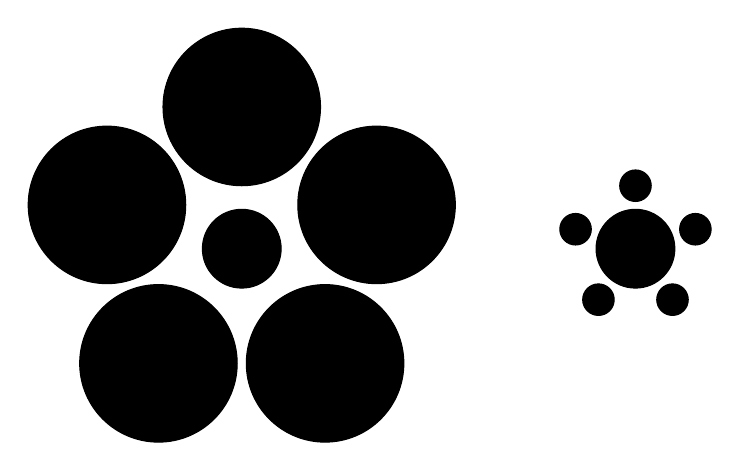
\begin{tikzpicture}
%% surrounded by big circles (looks smaller)
  \centercircle
  \foreach \a in {1,...,5}
    \filldraw (90+360/5*\a:1.8) circle(1);
%% surrounded by small circles (looks bigger)
  \begin{scope}[xshift=5cm]
    \centercircle
    \foreach \a in {1,...,5}
    \filldraw (90+360/5*\a:0.8) circle(0.2);
  \end{scope}
\end{tikzpicture}
\end{document}